\documentclass[a4paper,11pt,oneside]{report}
\usepackage[T1]{fontenc} % Fontes T1
\usepackage[utf8]{inputenc} % Input UTF8
\usepackage[backend=biber, style=ieee]{biblatex} % para usar bibliografia
\usepackage{csquotes}
\usepackage[portuguese]{babel} %Usar língua portuguesa
\usepackage{blindtext} % Gerar texto automaticamente
\usepackage[printonlyused]{acronym}
\usepackage{hyperref} % para autoref
\usepackage{graphicx}
\usepackage{setspace}
\usepackage{float}
\usepackage{indentfirst}

\bibliography{bibliografia}

\setlength{\parskip}{0.5cm}

\begin{document}
\onehalfspacing
%%
% Definições
%
\def\titulo{Mecânica - Cinemática e Dinâmica}
\def\data{DATA}
\def\autores{Autor1, Autor2}
\def\autorescontactos{(nmec1) autor1@ua.pt, (nmec2) autor2@ua.pt}
\def\versao{VERSAO}
\def\departamento{DEPARTAMENTO}
\def\empresa{EMPRESA}
\def\data{19 de dezembro de 2021}
\def\autores{Beatriz Oliveira, João Gaspar}
\def\autorescontactos{(108606) beatrizroliveira@ua.pt, (108807) j.gaspar@ua.pt}
\def\versao{1}
\def\departamento{Departamento de Engenharia de Telecomunicações e Informática}
\def\empresa{Universidade de Aveiro}
\def\logotipo{ua.pdf}
\def\codeua{Code UA: https://code.ua.pt/projects/infor2021-t3g62}
%
%%%%%% CAPA %%%%%%
%
\begin{titlepage}

\begin{center}
%
\vspace*{50mm}
%
{\Huge \titulo}\\ 
%
\vspace{10mm}
%
{\Large \empresa}\\
%
\vspace{10mm}
%
{\LARGE \autores}\\ 
%
\vspace{30mm}
%
\begin{figure}[h]
\center
\includegraphics{\logotipo}
\end{figure}
%
\vspace{30mm}
\end{center}
%
\begin{flushright}
\versao
\end{flushright}
\end{titlepage}

%%  Página de Título %%
\title{%
{\Huge\textbf{\titulo}}\\
{\Large \departamento\\ \empresa}
}
%
\author{%
    \autores \\
    \autorescontactos
}
%
\centering{\codeua}
\date{\data}
%
\maketitle

\pagenumbering{roman}

%%%%%% RESUMO %%%%%%
\begin{abstract}
Este trabalho assenta numa análise e reflexão dos movimentos efetuados num corpo (cinemática) e as suas respetivas forças (dinâmica), 
dando exemplos simples do quotidiano. 

A cinemática é a área da mecânica que estuda as situações que ocorrem a partir do instante em que um corpo inicia o seu estado de movimento,
desprezando as suas causas. A cinemática entende o movimento e propõe padrões matemáticos (equações e gráficos) que podem explicar e diferenciar o movimento. 
As formas mais comuns de estudo de movimento são: uniforme, uniformemente variado, circular uniforme e circular uniformemente variado. 

Na dinâmica procura-se entender as causas que originam um movimento. Como o movimento está sob a tensão de forças, podemos dizer que é o estudo das forças. 
As três leis de Newton são algumas das mais importantes fórmulas utilizadas nesta área da mecânica.

Este projeto aprofunda o estudo da mecânica nomeadamente movimentos de uma partícula num espaço a duas dimensões e também deslocações de sistemas de partículas. 
Conhecendo-se as forças que atuam numa partícula e sabendo a sua localização e a sua velocidade num dado instante, pode-se conhecer essas grandezas em qualquer instante, 
este conhecimento quando aplicado a situações do quotidiano, permite o desenvolvimento tecnológico que consequentemente ajuda o ser humano.
    
\end{abstract}

%%%%%% Agradecimentos %%%%%%
% Segundo glisc deveria aparecer após conclusão...
\renewcommand{\abstractname}{Agradecimentos}
\begin{abstract}
Para a realização deste trabalho contribuíram várias pessoas, 
que desde já queremos expressar o nosso enorme agradecimento. 

Em especial, queremos expressar a nossa gratidão para com o \textbf{Sr. 
Professor Óscar Pereira} por nos ter proporcionado as bases necessárias 
para a realização deste documento em \LaTeX.  
\end{abstract}


\tableofcontents
% \listoftables     % descomentar se necessário
% \listoffigures    % descomentar se necessário


%%%%%%%%%%%%%%%%%%%%%%%%%%%%%%%
\clearpage
\pagenumbering{arabic}

%%%%%%%%%%%%%%%%%%%%%%%%%%%%%%%%
\chapter{Introdução}
\label{chap.introducao}

Mecânica é uma parte da física que se centraliza no conhecimento do movimento 
e repouso dos corpos, estando eles ou não sob a ação de forças. A mecânica clássica 
divide-se em duas grandes áreas: cinemática e dinâmica.

A mecânica pode explicar desde o mais pequeno dos movimentos (de pessoas e carros) 
até o movimento mais significativo (dos planetas ao redor do Sol). Esta área é muito 
versátil e abrangente e, por isso, a escolhemos para desenvolver o nosso projeto de 
aprofundamento em \LaTeX.

Este documento está dividido em sete capítulos. Depois desta introdução, no Capítulo 
2 são apresentadas as equações da posição, as paramétricas e a trajetória descrita 
por um corpo; no Capítulo 3 é apresentado o deslocamento de um corpo assim com as 
suas equações de velocidade e aceleração; o Capítulo 4 refere-se à componente da 
aceleração; o Capítulo 5 evidencia os movimentos de uma partícula sob ação de uma 
força constante; o Capítulo 6 engloba os movimentos de corpos sujeitos a ligações 
e finalmente, no Capítulo 7 são apresentadas as conclusões do trabalho.


\chapter{Posição, equações paramétricas do movimento e trajétória}
\label{chap.posicao}

A \textbf{trajetória} do centro de massa de um corpo pode ser retilínea ou curvilínea.
Se a trajétória for retílinea, basta um único eixo cartesiano para caracterizar o movimento.
Desta forma aplica-se agora essa descrição para movimentos curvilíneos no plano e no espaço.

A \textbf{posição} de uma partícula  depende do referencial no qual o movimento é representado, e pode ser 
retratada por um vetor, de símbolo \(\vec{r}\), que é originário na origem do 
referencial e a sua extremidade sobre a partícula.

Num movimento retilíneo, como o de um corpo que desliza numa superfície plana com barreiras e que 
está num ponto \textbf{P} de coordenadas \textit{x} (\autoref{fig:corpo.1}), a posição do centro de massa pode escrever-se 
como \(\vec{r} = \textit{x} \times \vec{e_x}\), sendo \(\vec{e_x}\) o vetor unitário
cuja direção é a do eixo dos xx, apontando no sentido positivo desse eixo.

\begin{figure}[h]
    \center
    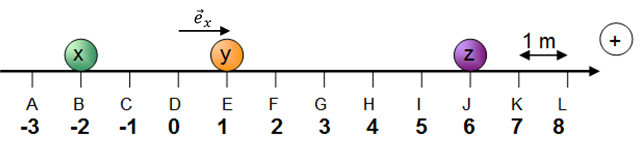
\includegraphics[height=50pt]{figuras/corpoposicao.png}
    \caption{Movimento retilíneo de um corpo.}
    \label{fig:corpo.1}
\end{figure}

Se o movimento descrito for curvilíneo como o do centro de massa de um 
carro a percorrer uma rotunda (\autoref{fig:corpo.2}), para descrever a sua posição serão necessárias duas coordenadas,
\textit{x} e \textit{y}. Definem-se os vetores unitários, \(\vec{e_x}\) e \(\vec{e_y}\), 
decompondo-se o vetor \(\vec{r}\) nestes eixos: \(\vec{r} = \textit{x} \times \vec{e_x} + \textit{y} \times \vec{e_y}\).

\begin{figure}[h]
    \center
    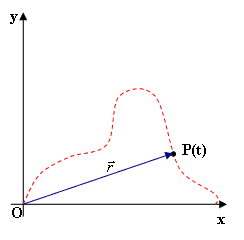
\includegraphics[height=150pt]{figuras/vet13.png}
    \caption{Movimento curvilíneo de um corpo.}
    \label{fig:corpo.2}
\end{figure}

O movimento curvilíneo a três dimensões (\autoref{fig:corpo.3}),
é um movimento mais complexo uma vez que são necessárias três coordenadas, \textit{x}, \textit{y} e \textit{z}, sendo o vetor posição
dado por \(\vec{r} = \textit{x} \times \vec{e_x} + \textit{y} \times \vec{e_y} + \textit{z} \times \vec{e_z}\).

\begin{figure}[h]
    \center
    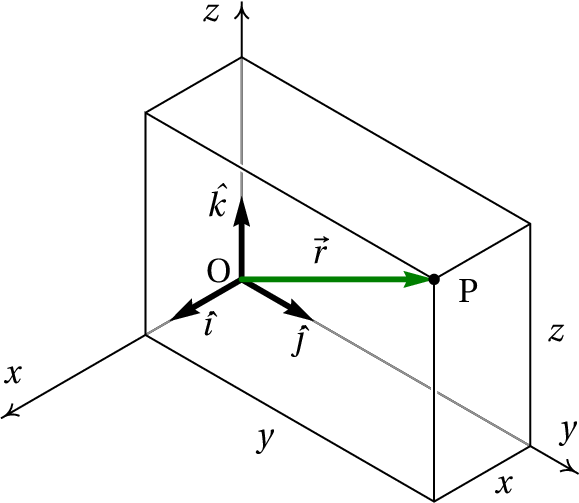
\includegraphics[height=150pt]{figuras/xyz.png}
    \caption{Movimento curvilíneo a três dimensões de um corpo.}
    \label{fig:corpo.3}
\end{figure}

As três equações referidas anteriormente, que indicam a variação de cada coordenada com o tempo,
podem ser designadas por \textbf{equações escalares} ou \textbf{paramétricas do movimento}.

A localização da partícula ao longo do tempo, também designada por \textbf{lei do movimento},
pode então ser representada por 
\[
\vec{r}(t) = x(t)\vec{e_x} + y(t)\vec{e_y} + z(t)\vec{e_z}
\]
O módulo de um vetor escreve-se \(| \vec{r}\vert \).

Pode-se resumir então as características do vetor posição:

\hrulefill
\begin{center}
    Posição, \(\vec{r}\)
\end{center}
\begin{itemize}
    \item Vetor com origem na origem do referencial e extremidade na partícula; depende do referencial em que é defenido.
    \item A sua expresão vetorial (designada por lei do movimento) é dada por:
   
     \(\vec{r}(t) = x(t)\vec{e_x}\) num movimento retilíneo;

     \(\vec{r}(t) = x(t)\vec{e_x} + y(t)\vec{e_y}\) num movimento curvilíneo no plano;

     \(\vec{r}(t) = x(t)\vec{e_x} + y(t)\vec{e_y} + z(t)\vec{e_z}\) num movimento curvilíneo no espaço.
    \item As sua projeções escalares, \textit{x}, \textit{y} e \textit{z}, podem diferenciar com o decorrer do tempo,
    tomando valores positivos, negativos ou nulos, sendo as funções
     \[
     x = x(t), y = y(t), z = z(t)
     \]
     designadas por \textbf{equações paramétricas do movimento}.
    \item O seu módulo (positivo) é dado por 
     \[
     r = | \vec{r}\vert = \sqrt{x^2 + y^2 + z^2}
     \]
     e indica a distância da partícula à origem do referencial.
\end{itemize}
\hrulefill

Qualquer \textbf{movimento curvilíneo} pode ser descrito numa formação 
de movimentos retilíneos em dois eixos (movimento num plano) ou em três eixos (movimento
no espaço).

Pode-se exemplificar com o movimento do centro de massa de uma bola lançada a partir de uma mesa horizontalmente
em queda livre. Este movimento curvilíneo, que se realiza num plano, pode ser visto
como a composição de um movimento segundo dois eixos (um eixo horizontal e um eixo vertical).

\begin{figure}[h]
    \center
    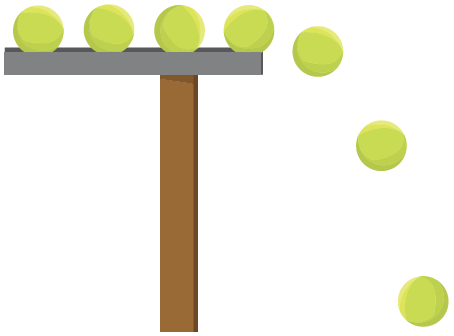
\includegraphics[height=150pt]{figuras/124.png}
    \caption{Lançamento horizontal de uma bola.}
    \label{fig:corpo.4}
\end{figure}

A representação estroboscópica no gráfico \(y(x)\) permite analisar o movimento
nos dois eixos e caracterizar o movimento em cada eixo como uniforme, acelerado ou retardado,
equiparando as distâncias percorridas entre posições sucessivas em intervalos de tempo iguais. 
Os movimentos em cada eixo são descritos pelas respetivas equações paramétricas, sendo possível
representá-los em gráficos posição-tempo (\autoref{fig:corpo.5}).

\begin{figure}[h]
    \center
    a) 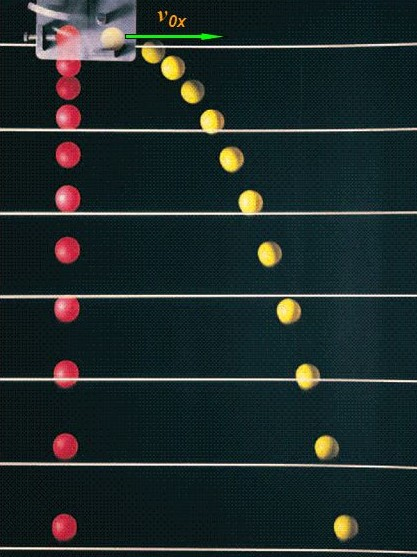
\includegraphics[height=80pt]{figuras/estroboscopica.jpg}
    b) 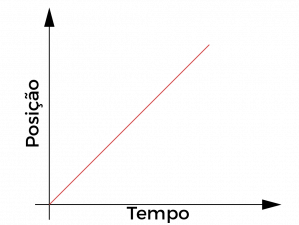
\includegraphics[height=80pt]{figuras/mvu.png}
    c) 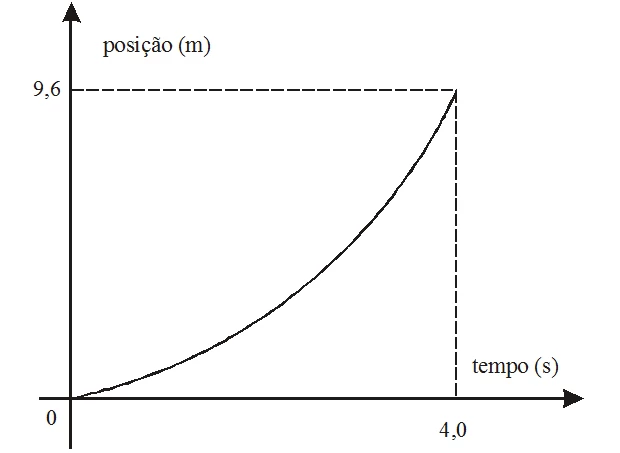
\includegraphics[height=80pt]{figuras/muva.png}
    \caption{a) Representação estroboscópica do movimento e sua decomposição em dois
    movimentos; b) Movimento uniforme no eixo horizontal: $x(t)=x_0+vt$; c) Movimento uniformemente
    acelerado: $y(t)=y_0+v_0t+\frac{1}{2}at^2 $.}
    \label{fig:corpo.5}
\end{figure}

A forma das equações paramétricas dos movimentos retilíneos em 
cada eixo permite a sua definição, como se descreve:

\begin{table}[H]
    \centering
    \begin{tabular}{|ll|l}
    \cline{1-2}
    \multicolumn{2}{|c|}{Equações paramétricas} &  \\ \cline{1-2}
    \multicolumn{1}{|l|}{\begin{tabular}[c]{@{}l@{}}Movimento uniforme \\ (aceleração nula)\end{tabular}} & \begin{tabular}[c]{@{}l@{}}A coordenada de posição é uma \\função polinomial do 1º grau em t. \\ Exemplo: \(x (t) = 5-10t\)\end{tabular} &  \\ \cline{1-2}
    \multicolumn{1}{|l|}{\begin{tabular}[c]{@{}l@{}}Movimento uniformemente variado \\ (aceleração constante)\end{tabular}} & \begin{tabular}[c]{@{}l@{}}A coordenada de posição é uma \\função polinomial do 2º grau em t. \\ Exemplo: \(y (t) = -2+10t-5t^2\)\end{tabular} &  \\ \cline{1-2}
    \multicolumn{1}{|l|}{\begin{tabular}[c]{@{}l@{}}Movimento variado \\ (aceleração variável)\end{tabular}} & \begin{tabular}[c]{@{}l@{}}A coordenada de posição é uma \\função polinomial de grau superior \\ a 2 em t. Exemplo: \(z (t) = 2-10^3\)\end{tabular} &  \\ \cline{1-2}
    \end{tabular}
    \caption{Caracterização dos movimentos conforme a forma das equações paramétricas.}
    \label{tabela}
\end{table}

A \textbf{equação da trajetória} de uma partícula obtém-se a partir das equações
paramétricas do movimento por remoção do parâmetro \textit{t}.

No exemplo da \autoref{fig:corpo.5}, se as equações paramétricas forem
\(x(t) = 10t\) e \(y(t) = 5-5t^2\), removendo o parâmetro \textit{t}
na equação \(x(t)\) e trocando-o na equação \(y(t)\) resultará \(5-5(\frac{x}{10} )^2\), o que
determina que a trajetória é uma parábola.

Como o resultado anterior é universal, conclui-se que se as equações paramétricas de um movimento forem uma do primeiro 
grau e outra do segundo grau, a trajetória será uma parábola.

\chapter{Deslocamento, velocidade média, velocidade e aceleração}
\label{chap.deslocamento}

O \textbf{deslocamento} de uma partícula, $\bigtriangleup\overrightarrow{r}$, relata a variação da sua posição num dado intervalo de tempo. 
Se ela se mover de uma posição \textbf{A} para uma posição \textbf{B}, o deslocamento será um vetor com origem em \textbf{A} e extremidade em \textbf{B}. 
Se traçarmos os vetores posição de \textbf{A}, $\overrightarrow{r_A}$,  e de \textbf{B}, $\overrightarrow{r_B}$,  de acordo com a regra da soma de vetores podemos escrever $\overrightarrow{r_B}=\overrightarrow{r_A}+\bigtriangleup\overrightarrow{r}$

\[
    \Leftrightarrow \bigtriangleup\overrightarrow{r}=\overrightarrow{r_B}-\overrightarrow{r_A}   
\]

Na \autoref{fig:corpo.6} podemos ver que \textbf{o módulo do vetor, $\bigtriangleup\overrightarrow{r}$  não é igual à distância percorrida sobre a trajetória}, $s$, entre A e B dada 
pelo comprimento do arco AB. Apenas quando a trajetória é retilínea e não há inversão de sentido do movimento é que o módulo 
do deslocamento coincide com a distância percorrida.

\begin{figure}[H]
    \center
    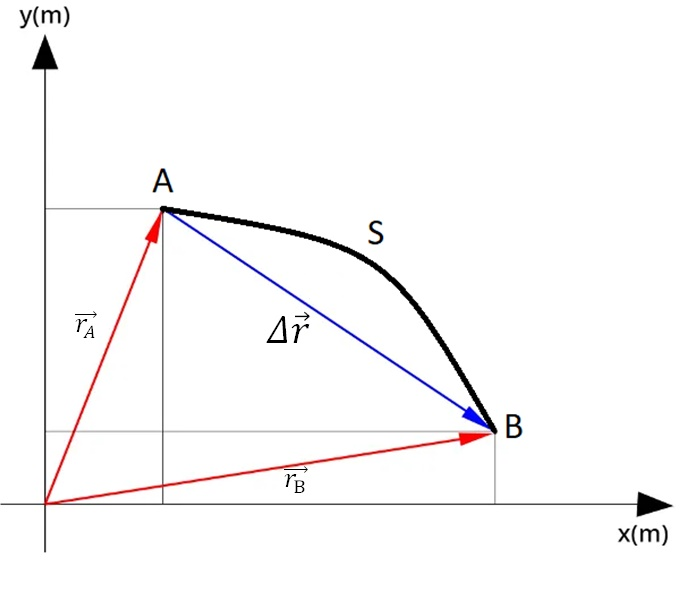
\includegraphics[height=170pt]{figuras/Fig 3.1.jpg}
    \caption{Trajetória de uma partícula e vetores posição, $\overrightarrow{r_A}$ e $\overrightarrow{r_B}$, vetor deslocamento, $\bigtriangleup\overrightarrow{r}$, e distância
    percorrida sobre a trajetória, $s$.}
    \label{fig:corpo.6}
\end{figure}


A \textbf{velocidade média} de uma partícula, $\overrightarrow{v_m}$  é o quociente entre o seu deslocamento entre duas posições e o correspondente 
intervalo de tempo:

\[
    \overrightarrow{v_m}=\frac{\bigtriangleup\overrightarrow{r}}{\bigtriangleup t}  
\]

A velocidade média indica se a partícula muda mais ou menos rapidamente de posição num dado intervalo de tempo. Como \textbf{$\bigtriangleup t$
tem sempre um valor positivo}, a direção e o sentido da velocidade média são as do vetor deslocamento.

Quando o ponto B se aproxima tanto de A que praticamente coincide com ele ($\bigtriangleup t$ é praticamente zero) 
a velocidade média “transforma-se” em \textbf{velocidade instantânea} ou, simplesmente, \textbf{velocidade}. A fórmula matemática da velocidade é:

\[
    \overrightarrow{v}=\lim_{\bigtriangleup t \to 0}   \frac{\bigtriangleup\overrightarrow{r}}{\bigtriangleup t} 
\]
que é equivalente a:
\[
    \overrightarrow{v}=\frac{d \overrightarrow{r}}{d t}  
\]

Ou seja, a velocidade é a derivada temporal do vetor posição (a derivada de uma função $f(t)$, em ordem à variável $t$, 
representa-se por $f'(t)$).

De acordo com as regras de derivação (soma e produto), e já que os vetores são \textbf{unitários} $\overrightarrow{e_x}$, $\overrightarrow{e_y}$ e $\overrightarrow{e_z}$ são constantes no tempo, 
a derivada da posição num referencial cartesiano $\overrightarrow{r}(t)=x(t)\overrightarrow{e_x}+y(t)\overrightarrow{e_y}+z(t)\overrightarrow{e_z}$, é representada por:
\[
   \overrightarrow{v}=\frac{d \overrightarrow{r}}{d t}=\frac{d x}{d t} \overrightarrow{e_x}+\frac{d y}{d t} \overrightarrow{e_y}+\frac{d z}{d t} \overrightarrow{e_z}
\]        

Por isso, a velocidade é uma função do tempo e escreve-se na forma:
\[
    \overrightarrow{v}(t)=v_x \overrightarrow{e_x}+v_y \overrightarrow{e_y}+v_z \overrightarrow{e_z}   
\] 

Com as componentes escalares da velocidade dadas por:
\[
    v_x=\frac{d x}{d t} \qquad v_y=\frac{d y}{d t} \qquad v_z=\frac{d z}{d t} 
\]

A \textbf{aceleração média} num dado intervalo de tempo é o quociente entre a variação de velocidade e o respetivo intervalo de tempo:
\[
    \overrightarrow{a_m}=\frac{\bigtriangleup\overrightarrow{v}}{\bigtriangleup t}  
\]

A direção e o sentido de $\overrightarrow{a_m}$ são os mesmos que os de $\bigtriangleup\overrightarrow{v} $, pois $\bigtriangleup t$ é sempre \textbf{positivo}.

Para conhecer a aceleração num dado instante, procede-se da mesma forma que na determinação da velocidade instantânea: 
parte-se da definição de aceleração média e considera-se o ponto \textbf{B tão próximo quanto possível de A}. A \textbf{aceleração instantânea} 
é dada por:
\[
    \overrightarrow{a}=\lim_{\bigtriangleup t\to 0} \frac{\bigtriangleup\overrightarrow{v}}{\bigtriangleup t}    
\]
ou 
\[
    \overrightarrow{a}=\frac{d \overrightarrow{v}}{d t}  
\]

que é a derivada temporal da velocidade. 

A aceleração, que é uma função do tempo, é dada por:
\[
    \overrightarrow{a}(t)=a_x\overrightarrow{e_x}+a_y\overrightarrow{e_y}+a_z\overrightarrow{e_z}    
\]
sendo:
\[
    a_x=\frac{d v_x}{d t} \qquad a_y=\frac{d v_y}{d t} \qquad a_z=\frac{d v_z}{d t}  
\]

Na \autoref{fig:corpo.7} mostra-se os vetores aceleração e velocidade do centro de massa de um automóvel que segue uma trajetória curvilínea: 
o aumento da distância percorrida em intervalos de tempo iguais e o aumento do módulo da velocidade revelam que o movimento 
é acelerado.

\begin{figure}[H]
    \center
    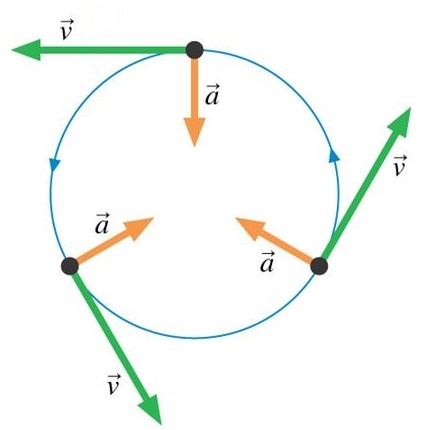
\includegraphics[height=170pt]{figuras/Fig 3.2.jpg}
    \caption{Vetores velocidade e aceleração num movimento curvilíneo acelerado.}
    \label{fig:corpo.7}
\end{figure}

Concluindo, há a possibilidade de descrever as trajetórias retilíneas e curvilíneas por meio de vetores (vetor velocidade 
e vetor aceleração)(\autoref{tab:tabela2}). 

\begin{table}[H]
    \begin{tabular}{lllll}
    \cline{1-2}
    \multicolumn{1}{|l|}{Trajetórias retilíneas}                                                                                                                                                         & \multicolumn{1}{l|}{Trajetórias curvilíneas}                                                                                                                                                                           &  &  &  \\ \cline{1-2}
    \multicolumn{1}{|l|}{\begin{tabular}[c]{@{}l@{}}$\vec a$ e $\vec v$ têm sempre a mesma direção, \\ que coincidem com a direção da \\ trajetória (podem ou não ter o \\ mesmo sentido).\end{tabular}} & \multicolumn{1}{l|}{\begin{tabular}[c]{@{}l@{}}$\vec a$ e $\vec v$ nunca têm a mesma direção: \\ $\vec a$ aponta sempre o interior da curva \\ e $\vec v$ é sempre tangente à curva em \\ cada ponto.\end{tabular}} &  &  &  \\ \cline{1-2}
                                                                                                                                                                                                         &                                                                                                                                                                                                                        &  &  &  \\
                                                                                                                                                                                                    &                                                                                                                                                                                                                        &  &  & 
    \end{tabular}
    \caption{Quadro-resumo sobre os vetores das trajetórias.}
    \label{tab:tabela2}
\end{table}

\chapter{Componentes tangencial e normal da aceleração}
\label{chap.componemtes}

As variações da velocidade de um corpo são provocadas por forças, 
que são estudadas na \textbf{dinâmica}.

A variação da velocidade pode ocorrer em módulo ou em direção ou
 ainda como no movimento do centro de massa de uma patinadora, 
 simultaneamente em módulo e direção.

\noindent \hrulefill
\begin{center}
    Efeito da força resultante na velocidade do centro de massa de um corpo
\end{center}
\begin{table}[h]
    \centering
    \begin{tabular}{lll}
    \multicolumn{1}{l|}{\begin{tabular}[c]{@{}l@{}}$\overrightarrow{F_R}$ tem a direção de $\vec v$: a trajetória \\ é retilínea. O movimento será \\ acelerado, se $\overrightarrow{F_R}$ e $\vec v$  tiverem \\ o mesmo sentido, ou retardado \\ se tiverem sentidos opostos.\end{tabular}} & \begin{tabular}[c]{@{}l@{}}$\overrightarrow{F_R}$ não tem a direção de $\vec v$: a \\ trajetória é curvilínea. Se $\overrightarrow{F_R}$ e $\vec v$ \\ forem perpendiculares, o movimento \\ será uniforme; será acelerado \\ se fizerem um ângulo inferior \\ a $90^\circ$; será retardado \\ se esse ângulo for superior a $90^\circ$.\end{tabular} &  \\
    \end{tabular}
    \caption{Efeito da força resultante na velocidade.}
    \label{tab:tabela3}
\end{table}
\hrulefill

Num movimento curvilíneo, como o vetor aceleração está direcionado para
o interior da curva, pela Segunda Lei de Newton, $\overrightarrow{F_R}=m\vec a$, 
conclui-se que o mesmo acontece com o vetor força resultante, $\overrightarrow{F_R}$,
pois este tem a direção e o sentido da aceleração. Por vezes, é conveniente 
decompor a força resultante em duas componentes:

\begin{enumerate}
    \item \textbf{Componente tangencial da força resultante, $\overrightarrow{F_t}$}: tem a direção da velocidade (é tangente à trajetória), o mesmo sentido ou sentido oposto, e provoca uma variação no módulo da velocidade;
    \item \textbf{Componente normal da força resultante, $\overrightarrow{F_n}$ (também designada por força centrípeta, $\overrightarrow{F_c}$)}: é normal (perpendicular) à velocidade, aponta para o centro da curva (é centrípeta), e provoca uma variação da direção da velocidade. Apenas existe nos movimentos curvilíneos, pois só nestes a direção da velocidade varia.
\end{enumerate}

Como as variações da velocidade são descritas pela aceleração, $\vec a$, 
e atendendo à Segunda Lei de Newton, também se pode decompor a aceleração 
em duas componentes, a \textbf{componente tangencial}, $\overrightarrow{a_t}$, 
e a \textbf{componente normal}, $\overrightarrow{a_n}$an: 

\[
\vec a = \overrightarrow{a_t} + \overrightarrow{a_n}
\]

Estas componentes relacionam-se com as componentes tangencial e
normal da força resultante atendendo à Segunda Lei de Newton:

\[
\overrightarrow{F_t} = m\overrightarrow{a_t} 
\]
\[
\overrightarrow{F_n} = m\overrightarrow{a_n}
\]

A \autoref{fig:corpo8} representa, um ponto da trajetória, o vetor velocidade 
e o vetor aceleração, assim como a respetiva componente tangencial e 
normal.

\begin{figure}[H]
    \center
    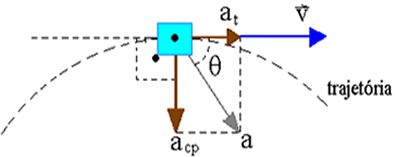
\includegraphics[height=100pt]{figuras/avv.jpg}
    \caption{A aceleração é a soma da componemte tangencial e da componemte normal.
    A velocidade é sempre tangencial à trajetória.}
    \label{fig:corpo8}
\end{figure}

A \autoref{fig:corpo8} permite concluir que, quando o movimento é retardado, como no 
ponto \textbf{A}, o ângulo $\theta$ entre os vetores aceleração e velocidade 
é superior a $90^\circ$; quando o movimento é acelerado, como nos pontos \textbf{B} 
e \textbf{C}, o ângulo $\theta$ entre os vetores velocidade e aceleração é inferior 
a $90^\circ$. 

A derivada temporal do módulo da velocidade é a componente tangencial da 
aceleração já que mede a variação do módulo a velocidade num dado instante:

\[
a_t = \frac{dv}{dt}
\]

\noindent pode-se ainda calcular a componente tangencial da aceleração pela expressão: 

\[
a_t = a\cos \theta
\]

Note-se que, se o ângulo $\theta$ for maior do que $90^\circ$, a componente 
tangencial da aceleração será negativa, o que significa que o movimento será 
retardado.

A componente tangencial da aceleração permite classificar os movimentos em 
uniformes, uniformemente variados e variados:

\begin{itemize}
    \item Movimentos uniformes
     \begin{itemize}
     \item $a_t = O$ (o módulo da velocidade não varia)
     \end{itemize}
    \item Movimentos uniformemente variados
    \begin{itemize}
     \item $a_t = constante$ (o módulo da velocidade tem variação uniforme com o tempo)
    \end{itemize}
    \item Movimentos variados
     \begin{itemize}
     \item $a_t \ne constante$ (o módulo da velocidade varia de forma não uniforme com o tempo)
    \end{itemize}
\end{itemize}

A componente normal da aceleração é dada pela expressão

\[
a_n = \frac{v^2}{r}
\]

\noindent em que o símbolo \textit{r} representa o raio de curvatura.

A Fig.x representa a componente normal da aceleração que também pode ser 
calculada pela expressão:

\[
a_n = a\sin\theta
\]

Numa trajetória circular, o raio de curvatura, r, que corresponde ao raio da
circunferência. Nas outras curvas, para cada ponto atribui-se o \textbf{raio de curvatura} 
como o raio do arco circular que mais se aproxima da curva nesse ponto (\autoref{fig:corpo9}). 
O raio de curvatura é pequeno para curvas «fechadas» e grande para curvas «abertas», 
tendendo para infinito se a trajetória se aproximar de uma reta.

\begin{figure}[H]
    \center
    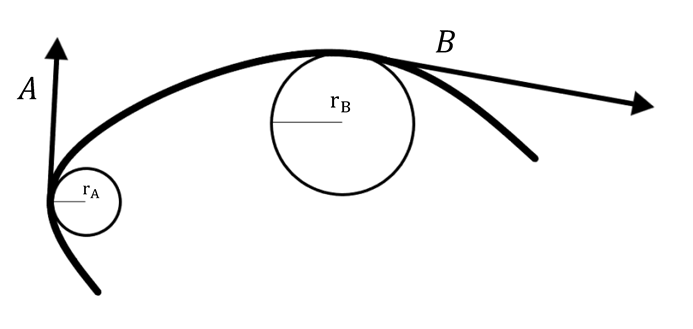
\includegraphics[height=100pt]{figuras/rdc.png}
    \caption{O raio de curvatura é menor numa curva mais pequena, como é o caso da posição A.}
    \label{fig:corpo9}
\end{figure}

A expressão da aceleração normal, $\frac{v^2}{r}$, indica que, quanto maior 
for a velocidade com que um automóvel faz uma curva, maior será a sua aceleração
normal.

Se a curva for apertada (menor raio), a aceleração normal também será maior 
para o mesmo valor da velocidade. Posto isto, terá de ser maior a componente 
normal da força resultante. Se essa força não for minimamente intensa, o automóvel 
não fará a curva.

Como as componentes tangencial e normal da aceleração permitem conhecer o tipo de 
movimento, é útil definir dois eixos perpendiculares com origem na partícula, um 
com a direção da velocidade (eixo tangencial) e outro com a direção perpendicular 
e dirigido para o centro de curvatura (eixo normal), cujos vetores unitários são, 
respetivamente, $\vec e_t$ e $\vec e_n$.

Neste sistema de eixos ligado à partícula, a expressão do vetor aceleração é:

\[
\vec a = a_t\vec e_t + a_n\vec e_n
\]

\noindent sendo o respetivo módulo dado por: 

\[
a = \sqrt{a_{t}^{2}+a_{n}^{2}}
\]

\chapter{Movimentos sob a ação de uma força resultante constante}
\label{chap.movimentos}

Um corpo no qual atua uma mesma força resultante pode adquirir \textbf{movimentos 
com trajetórias diferentes}. Isto acontece porque, embora a força resultante 
seja igual, as condições iniciais - a posição e a velocidade iniciais - 
são diferentes.

Vejamos o exemplo de uma bola que roda, presa a um fio, numa trajetória 
circular num plano vertical. \textbf{Não tendo em conta a resistência do ar}. 
Se fio se partir, como a bola tem uma certa velocidade no instante da rutura, 
ela passará a ter um movimento em \textbf{queda livre} pois a única força que nela 
atua será o seu \textbf{peso}. No entanto, a forma da trajetória que a bola fará vai 
depender da posição no instante de rutura do fio, pois \textbf{em diferentes posições 
existirão diferentes velocidades do centro de massa da bola}.

Note-se que corpos com igual velocidade inicial, mas sujeitos a uma força 
resultante diferente também formam trajetórias diferentes, ou seja, 
\textbf{a trajetória depende ao mesmo tempo da força resultante, da posição e 
velocidade iniciais}.

Efetuemos para dois movimentos comuns: o {\Large o lançamento horizontal} e o 
{\Large lançamento oblíquo}.

Num lançamento horizontal o projétil tem velocidade inicial horizontal. 
É o caso de uma bola que cai quando lançada do tampo de uma mesa.

Abaixo escrevem-se as equações paramétricas do movimento
e as componentes escalares da velocidade.

\hrulefill
\begin{center}
    \textbf{Lançamento horizontal}
\end{center}
\begin{itemize}
\centering
    \item[] $a_x = 0$ e $a_y = -g$
    \item[$\rightarrow$] Condições inicias:
    \begin{enumerate}
        \item $x_0 = 0$ e $y_0 = h$
        \item $v_{0x} = v_0$ e $v_{0y} = 0$
    \end{enumerate}
    \item[$\rightarrow$] Equações:
    \begin{enumerate}
        \item $x(t) = v_0 t$ e $y(t) = h - \frac{1}{2} g t^2$
        \item $v_x = v_0$ e $v_y (t) = -g t$
        \item sendo $v = \sqrt{v_{x}^{2} + v_{y}^{2}}$
    \end{enumerate}
\end{itemize}
\hrulefill

Verifique-se que a componente escalar vertical {\Large cresce}, pois, o movimento 
é uniformemente acelerado nesta direção, enquanto a componente escalar 
horizontal permanece igual, pois o movimento é uniforme na direção horizontal.

Ao remover a variável $t$ nas equações paramétricas, obtém-se a equação da 
trajetória, $y = h - \frac{1}{2}g\frac{x}{v_0}^2$, que é a equação de uma \textbf{parábola}.

O tempo de queda dá-se pela equação $y(t) = h - \frac{1}{2}gt^2$ fazendo $y = 0$:

\[
t = \sqrt{\frac{2h}{g}}
\]

Esta expressão mostra que \textbf{o tempo de queda depende da altura de queda}, $h$, 
mas não da velocidade inicial, $v_0$. Ou seja, uma bola lançada horizontalmente 
ou deixada cair da mesma altura demora o mesmo tempo a atingir o solo, pois os 
movimentos na direção vertical são os mesmos: a componente escalar vertical da 
posição, em cada instante, é a mesma.

O alcance do projétil, que é a distância máxima percorrida horizontalmente, 
consegue-se substituindo o tempo de queda na equação $x(t)=v_0t$, obtendo-se:

\[
x_{max} = v_0\sqrt{\frac{2h}{g}}
\]

Esta expressão permite deduzir que, para a mesma altura de queda, \textbf{quanto 
maior for a velocidade inicial maior será o alcance}.

Poderando agora o lançamento oblíquo de um projétil, ou seja, aquele em que 
a velocidade inicial é oblíqua, fazendo um certo ângulo, $\theta$, com a direção horizontal.

Ao contrário do lançamento horizontal, neste lançamento \textbf{a velocidade inicial 
tem duas componentes}: uma horizontal e outra vertical.

Na estrutura abaixo escrevem-se as equações paramétricas dos movimentos,
assim como as componentes escalares da velocidade.

\hrulefill
\begin{center}
    \textbf{Lançamento oblíquo}
\end{center}
\begin{itemize}\label{}
\centering
    \item[] $a_x = 0$ e $a_y = -g$
    \item[$\rightarrow$] Condições inicias:
    \begin{enumerate}
        \item $x_0 = 0$ e $y_0 = 0$
        \item $v_{0x} = v_0 \cos \theta$ e $v_{0y} = v_0 \sin \theta$
    \end{enumerate}
    \item[$\rightarrow$] Equações:
    \begin{enumerate}
        \item $x(t) = v_0 \cos \theta t $ e $y(t) = v_0 \sin \theta t - \frac{1}{2} g t^2$
        \item $v_x = v_0 \cos \theta$ e $v_y  = v_0 \sin \theta -g t$
        \item sendo $v = \sqrt{v_{x}^{2} + v_{y}^{2}}$
    \end{enumerate}
\end{itemize}
\hrulefill

Como mostra acima, o \textbf{módulo da componente escalar vertical da velocidade}, 
$v_y$ {\scriptsize diminui} na subida e {\Large aumenta} na descida, cortando-se mutuamente no ponto 
de {\Large altura máxima}. Fazendo $v_y = O$ na equação $v_y = v_0 \sin \theta - gt$ 
obtém-se o tempo de subida projétil:

\[
t_{subida} = \frac{v_0 \sin \theta}{g}
\]

Tendo em conta o caso particular de um projétil que volta ao plano horizontal 
de onde foi lançado. \textbf{O tempo de subida é igual ao tempo de descida}, por isso o 
tempo de voo - tempo que o projétil permanece no ar - é o dobro do tempo de subida:

\[
t_{voo} = 2\frac{v_0 \sin \theta}{g}
\]

Pode-se determinar uma expressão para a {\Large altura máxima} substituindo-se o tempo 
de subida, $t_{subida} = \frac{v_o \sin \theta}{g}$, na equação $y(t) = v_0 \sin \theta t - \frac{1}{2} g t^2$ 
e obtendo-se:

\[
y_{max} = \frac{v_{0}^{2} \sin^2 \theta}{2g}
\]

Do mesmo modo se define uma expressão para o alcance do projétil substituindo 
o tempo de voo, $t_{voo} = 2 \frac{v_0 \sin \theta}{g}$, na equação $x(t) = v_0 \cos \theta t$, 
obtendo-se:

\[
A = \frac{v_{0}^{2} \sin 2 \theta}{g}
\]

\chapter{Movimentos de corpos sujeitos a ligações}
\label{chap.ligacoes}

Analisa-se os movimentos de corpos sujeitos a uma força resultante contínua 
e, mais precisamente, movimentos de projéteis que apenas estão sujeitos ao seu 
peso.

Mas há corpos que estão ligados a outros, havendo forças que formem essas 
ligações. Estas forças chamam-se \textbf{forças de ligação}.

É o caso, por exemplo, de corpos suspensos de correntes, como num “slingshot” 
(\autoref{fig:corpo10}). Tendo em conta que o conjunto de correntes é equivalente a só fio, 
a força que esse fio executa sobre a cadeira, cuja direção coincide com a do fio, 
é a tensão, $\vec T$. Esta força garante a ligação entre a cadeira e o fio: diz-se 
que a \textbf{tensão} é uma \textbf{força de ligação}. A sua intensidade depende do 
peso do conjunto que roda \textit{(pessoa + cadeira)}: quanto maior for o peso, maior 
será a tensão.

\begin{figure}[H]
    \center
    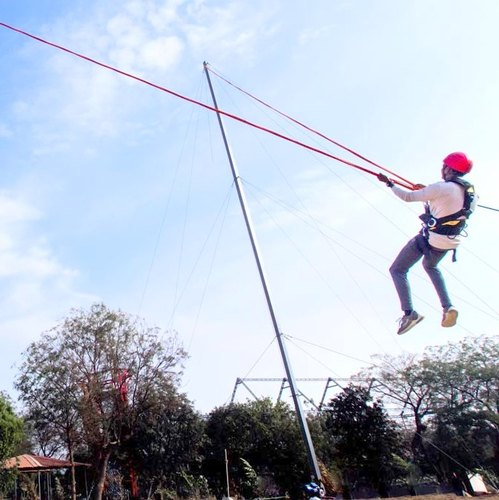
\includegraphics[height=100pt]{figuras/hss.jpg}
    \caption{Slingshot.}
    \label{fig:corpo10}
\end{figure}

Outro exemplo de força de Ligação é a força exercida sobre um corpo por um plano 
(horizontal, inclinado, etc), perpendicularmente a este: a força normal, N. Esta 
força restringe a trajetória do corpo, impedindo o movimento do corpo na direção 
perpendicular ao plano de apoio. outro exemplo, é o caso da força normal exercida 
num carrinho de uma montanha-russa (\autoref{fig:corpo11}).

\begin{figure}[H]
    \center
    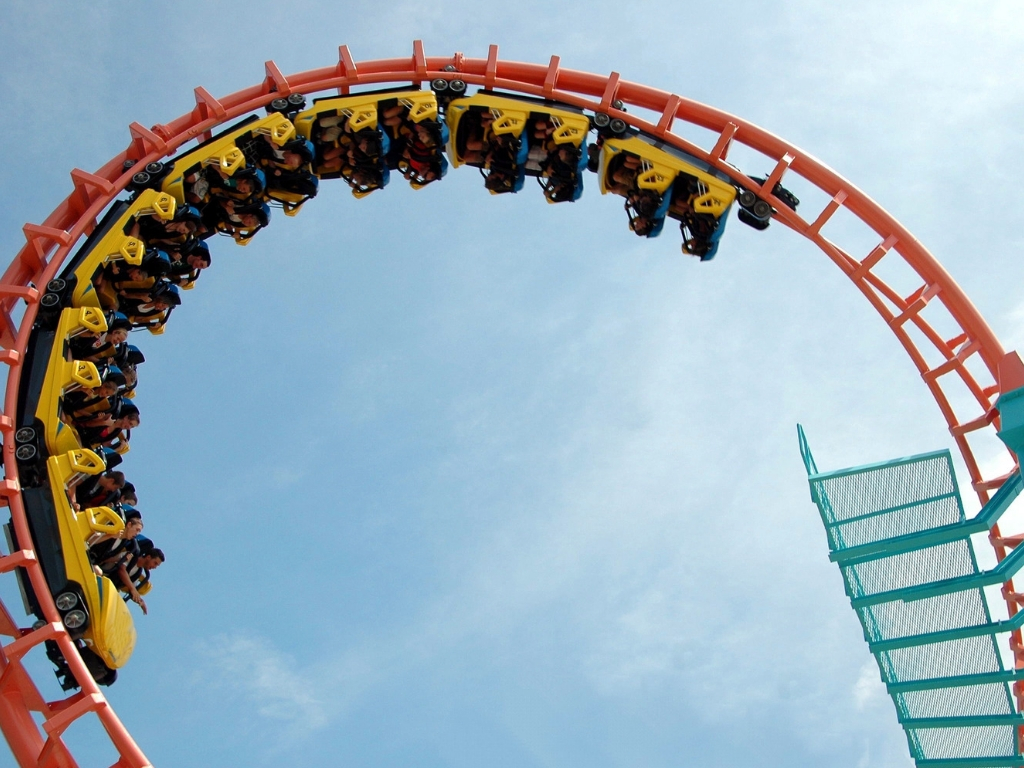
\includegraphics[height=100pt]{figuras/mr.jpg}
    \caption{Montanha-russa.}
    \label{fig:corpo11}
\end{figure}

Pode-se analisar alguns movimentos retilíneos e circulares sujeitos a ligações, 
na privação de forças de atrito, de maneira a calcular as intensidades da tensão, 
$\vec T$, e da força normal, $\vec N$.

\begin{center}
    Exemplo 1 - Movimento retilíneo de um sistema de corpos
\end{center}

Consegue-se analisar o movimento de dois esquiadores, agarrados por uma corda 
(ou fio), sendo um puxado por uma corda com uma força constante $\vec F$ sobre 
uma superfície onde é desprezável a força de atrito. 

Abaixo está descrita a situação anterior (\autoref{fig:corpo12}). Há três corpos em movimento: o corpo A, o 
corpo B e o fio que os une. Se a massa do fio for considerada nula, 
isto é, muito menor do que a massa dos restantes corpos, pode-se ignorar o peso do 
fio.

\begin{figure}[H]
    \centerline{\fbox{Dois corpos ligados por um fio}}
    \center
    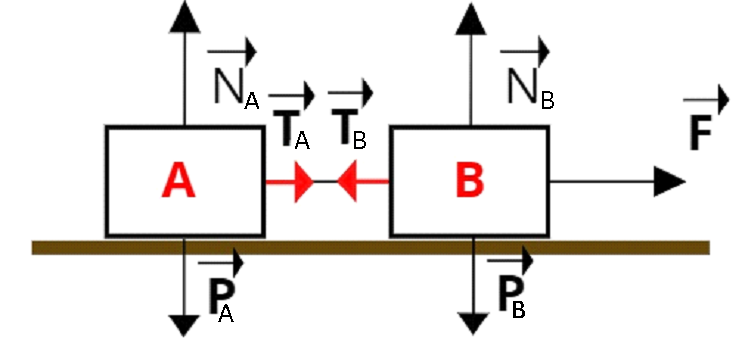
\includegraphics[height=100pt]{figuras/dabm.png}
    \caption{$\vec {T_B}$: força com que o fio (que liga os corpos) puxa o 
    corpo \textbf{B}. $\vec {P_B}$: peso de \textbf{BA}, exercido pela Terra. 
    $\vec {N_B}$: força normal exercida pelo plano de apoio.}
    \label{fig:corpo12}
\end{figure}


Aplicando a Segunda Lei de Newton vem, $F_x = ma$ e $F_y = 0$. Como não há forças 
segundo o eixo dos $yy$ e $m_{fio} \approx O$, obtém-se:

$F_x = m_{corda}a_x \Rightarrow T'_A - T'_B = 0 \Leftrightarrow T'_A = T'_B (com m_{fio} \approx 0)$

Em suma, sempre que a massa de um fio (ou corda) for quase insignificante, a tensão 
ao longo do fio tem a mesma intensidade.

Pode-se então escrever $T'_B = T'_A = T$. Mas, como $\vec{T'_B}$ e $\vec{T'_A}$ formam 
pares ação-reação com, respetivamente, $\vec{T_A}$ e $\vec{T_B}$, também se escreve

\[
T_B = T_A = T (com \ m_{fio}\approx0)
\]

\noindent \hrulefill
\begin{center}
    Corpo A:
\end{center}
\[
\left\{
\begin{array}{cl}
F_x & = ma_x \\
F_y & = 0
\end{array}
\Leftrightarrow
\right.
\left\{
\begin{array}{cl}
F \cos\theta - T & = m_Aa \\
F \sin \theta + N_A - P_A & = 0
\end{array}
\right.
\]
\begin{center}
    Corpo B:
\end{center}
\[
\left\{
\begin{array}{cl}
F_x & = ma_x \\
F_y & = 0
\end{array}
\Leftrightarrow
\right.
\left\{
\begin{array}{cl}
T & = m_Ba \\
N_B - P_B & = 0
\end{array}
\right.
\]
\hrulefill

Acima escreve-se a expressão da Segunda Lei de Newton para os corpos A e B.

As segundas equações de cada sistema permitem calcular a intensidade das respetivas 
forças normais: $N_A = P_A - F \sin \theta$ e $N_B = P_B$.

As equações restantes formam o sistema:

\[
\left\{
\begin{array}{cl}
F \cos \theta - T & = m_Aa \\
T & = m_Ba
\end{array}
\right.
\]

\noindent o qual possibilita obter a aceleração, a, com que se move o conjunto e o 
valor da tensão, $T$, a partir da intensidade da força, $F$, que puxa o corpo A e do 
ângulo $\theta$ (cujos valores são conhecidos): 

\[
a = \frac{F\cos\theta}{m_A+m_B} \qquad T = \frac{m_B}{m_A+m_B}
\]

\begin{center}
    Exemplo 2 - Movimento circular num plano vertical: a montanha-russa
\end{center}

Analisando o movimento de um carrinho numa montanha-russa, supondo que não existe 
um mecanismo de segurança que impeça a projeção do carrinho.

Analisando o movimento nas posições A, B, C e D (\autoref{fig:corpo13}), supondo que as últimas 
três posições estão sobre o mesmo arco de circunferência. As forças que se realizam 
sobre o carrinho são sempre as mesmas (contínuas): o peso, que é uma força de intensidade 
constante, e a força normal, que é variável em direção e intensidade.

\begin{figure}[H]
    \center
    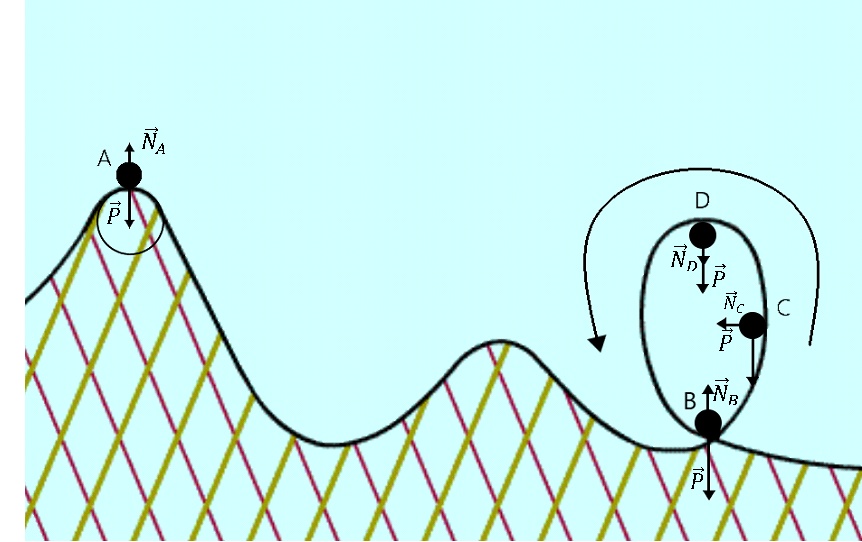
\includegraphics[height=100pt]{figuras/mvmr.png}
    \caption{Movimento de corpo numa montanha-russa quando se desloca por A, B, C e D}
    \label{fig:corpo13}
\end{figure}

Como a trajetória é redonda, deve-se usar um referencial ligado à partícula. Para cada 
posição, tem-se de ponderar três eixos: o tangencial, designado por $t$ e o normal, 
designado por $n$. Como não há nenhuma força na direção do eixo dos $zz$, $F_z=0$.

Escrevendo estas equações para cada ponto do carrinho atendendo ao raio de curvatura, 
que é r para a posição A e R para as posições B, C e D.

Para a posição A, vem: 

\[
\left\{
\begin{array}{cl}
F_t & = m_at \\
F_n & = m_an
\end{array}
\right.
\Rightarrow
\left\{
\begin{array}{cl}
0 & = m_at \\
P - N_A & = m\frac{v_{A}^{2}}{r}
\end{array}
\right.
\Rightarrow
\left\{
\begin{array}{cl}
a_t & = 0 \\
N_A & = P - m\frac{v_{A}^{2}}{r}
\end{array}
\right.
\]

Da primeira equação, concluímos que a aceleração tangencial é nula em A.

A segunda equação permite:
\begin{enumerate}
    \item calcular a intensidade da força normal, $\vec N$, conhecida a velocidade em \textbf{A};
    \item verificar que tem de existir a condição $N_A < P$, pois o segundo membro da equação, $m\frac{v_{A}^{2}}{r}$, é sempre positivo.
\end{enumerate}

Uma curva só é feita quando há uma componente centrípeta da resultante das forças a 
dirigir-se para o centro de curvatura. Por este motivo, \textbf{a intensidade da força 
que aponta para o centro da curvatura tem de ser maior do que a intensidade da força que 
aponta para fora}.

Como a intensidade da força normal é sempre positiva, $N_A > 0$, o caso limite ocorre para 
$N_A = 0$, ou seja, quando o plano não exerce força sobre o corpo. Nesta situação, o corpo 
fica prestes a entrar em voo de projétil, porque apenas atua o seu peso. Por isso tem de se 
verificar:

\[
N_A > 0 \Rightarrow P - m\frac{v_{A}^{2}}{r} > 0 \Leftrightarrow mg > m\frac{v_{A}^{2}}{r} \Leftrightarrow v_A < \sqrt{rg}
\]

Ou seja, a condição de segurança em A é que o módulo da velocidade seja inferior 
a $\sqrt{rg}$, ou seja o raio de curvatura é decisivo.

Para a posição B, as equações são: 

\[
\left\{
\begin{array}{cl}
F_t & = m_at \\
F_n & = m_an
\end{array}
\right.
\Rightarrow
\left\{
\begin{array}{cl}
0 & = m_at \\
N_B - P & = m\frac{v_{B}^{2}}{R}
\end{array}
\right.
\Rightarrow
\left\{
\begin{array}{cl}
a_t & = 0 \\
N_B & = P + m\frac{v_{B}^{2}}{R}
\end{array}
\right.
\]

Da primeira equação concluímos que a aceleração tangencial é nula em B.

A segunda equação permite:

\begin{enumerate}
    \item calcular a intensidade da força normal, $\vec N$, conhecida a velocidade em \textbf{B};
    \item verificar que a força normal nesta posição é sempre maior do que o peso, pois $P + m\frac{v_{B}^{2}}{R}$ é sempre positivo. Então, a segurança está garantida na posição B. No entanto, se a velocidade for demasiado alta, a força normal poderá ter uma intensidade tão grande que incomoda os passageiros.
\end{enumerate}

Para a posição C, as equações são:

\[
\left\{
\begin{array}{cl}
F_t & = m_at \\
F_n & = m_an
\end{array}
\right.
\Rightarrow
\left\{
\begin{array}{cl}
-P & = m_at \\
N_C & = m\frac{v_{C}^{2}}{R}
\end{array}
\right.
\Rightarrow
\left\{
\begin{array}{cl}
a_t & = -g \\
N_C & = m\frac{v_{C}^{2}}{R}
\end{array}
\right.
\]

Na posição D, as equações são:

\[
\left\{
\begin{array}{cl}
F_t & = m_at \\
F_n & = m_an
\end{array}
\right.
\Rightarrow
\left\{
\begin{array}{cl}
0 & = m_at \\
N_D + P & = m\frac{v_{D}^{2}}{R}
\end{array}
\right.
\Rightarrow
\left\{
\begin{array}{cl}
a_t & = 0 \\
N_D & = m\frac{v_{D}^{2}}{R} - P
\end{array}
\right.
\]

A segunda equação permite obter a condição de segurança em D, pois tem de se verificar: 

\[
N_D > 0 \Leftrightarrow m\frac{v_{D}^{2}}{R} - P > 0 \Leftrightarrow m\frac{v_{D}^{2}}{R} > mg \Leftrightarrow v_D > \sqrt{Rg}
\]

Ou seja, na posição de altura máxima do arco, o carrinho tem de ter uma velocidade 
mínima para não cair, que submete-se ao raio de curvatura.

\chapter*{Contribuições dos autores}
Nós consideramos que o trabalho foi bem distribuído entre nós. Começamos, ambos, 
por uma pesquisa prévia bastante abrangente sobre o assunto (mecânica). 
Em seguida optamos por distribuirmos os tópicos que iriamos mencionar neste trabalho 
por ambos de igual forma, para que fosse mais fácil, cada um de nós se focar nos seus 
próprios temas. A comunicação foi algo indispensável neste projeto, pois assim 
conseguimos ajudarmo-nos mutuamente nos problemas que eventualmente nos iria aparecendo. 

Beatriz Oliveira \ac{bo} - Realizou os agradecimentos, a introdução, o resumo e os capítulos 3 e 5.
João Gaspar \ac{jg} - Realizou a capa, página de título, os capítulos 2, 4 e 6, os acrónimos e a bibliografia.

Deste modo, ambos achamos que estivemos, cada um, 50\% presentes neste trabalho.


%%%%%%%%%%%%%%%%%%%%%%%%%%%%%%%%%
\chapter*{Acrónimos}
\begin{acronym}
\acro{bo}[BO]{Beatriz Oliveira}
\acro{jg}[JG]{João Gaspar}
\end{acronym}

% para usar escrever \ac{nome}

%%%%%%%%%%%%%%%%%%%%%%%%%%%%%%%%%
\printbibliography

\end{document}
